\documentclass{article} % For LaTeX2e
\usepackage{nips14submit_e,times}
\usepackage{amsmath}
\usepackage{amsthm}
\usepackage{amssymb}
\usepackage{mathtools}
\usepackage{hyperref}
\usepackage{url}
\usepackage{algorithm}
\usepackage[noend]{algpseudocode}
%\documentstyle[nips14submit_09,times,art10]{article} % For LaTeX 2.09

\usepackage{bbm}
\usepackage{graphicx}
\usepackage{caption}
\usepackage{subcaption}
\usepackage{MnSymbol}

\def\eQb#1\eQe{\begin{eqnarray*}#1\end{eqnarray*}}
\def\eQnb#1\eQne{\begin{eqnarray}#1\end{eqnarray}}
\providecommand{\e}[1]{\ensuremath{\times 10^{#1}}}
\providecommand{\pb}[0]{\pagebreak}
\DeclarePairedDelimiter\ceil{\lceil}{\rceil}
\DeclarePairedDelimiter\floor{\lfloor}{\rfloor}

\newcommand{\E}{\mathrm{E}}
\newcommand{\Var}{\mathrm{Var}}
\newcommand{\Cov}{\mathrm{Cov}}
\newcommand\eqD{\stackrel{\mathclap{\normalfont\mbox{d}}}{=}}

\def\Qb#1\Qe{\begin{question}#1\end{question}}
\def\Sb#1\Se{\begin{solution}#1\end{solution}}

\newenvironment{claim}[1]{\par\noindent\underline{Claim:}\space#1}{}
\newtheoremstyle{quest}{\topsep}{\topsep}{}{}{\bfseries}{}{ }{\thmname{#1}\thmnote{ #3}.}
\theoremstyle{quest}
\newtheorem*{definition}{Definition}
\newtheorem*{theorem}{Theorem}
\newtheorem*{lemma}{Lemma}
\newtheorem*{question}{Question}
\newtheorem*{preposition}{Preposition}
\newtheorem*{exercise}{Exercise}
\newtheorem*{challengeproblem}{Challenge Problem}
\newtheorem*{solution}{Solution}
\newtheorem*{remark}{Remark}
\usepackage{verbatimbox}
\usepackage{listings}
\usepackage{mathrsfs}
\title{ProbLimI: \\
Problem Set XII}


\author{
Youngduck Choi \\
CIMS \\
New York University\\
\texttt{yc1104@nyu.edu} \\
}


% The \author macro works with any number of authors. There are two commands
% used to separate the names and addresses of multiple authors: \And and \AND.
%
% Using \And between authors leaves it to \LaTeX{} to determine where to break
% the lines. Using \AND forces a linebreak at that point. So, if \LaTeX{}
% puts 3 of 4 authors names on the first line, and the last on the second
% line, try using \AND instead of \And before the third author name.

\newcommand{\fix}{\marginpar{FIX}}
\newcommand{\new}{\marginpar{NEW}}

\nipsfinalcopy % Uncomment for camera-ready version

\begin{document}


\maketitle

\begin{abstract}
This work contains solutions to the exercises of the problem set XII. The
chosen problems are 2,3,4.
\end{abstract}

\bigskip

\begin{question}[2]
\hfill
\begin{figure}[h!]
  \centering
    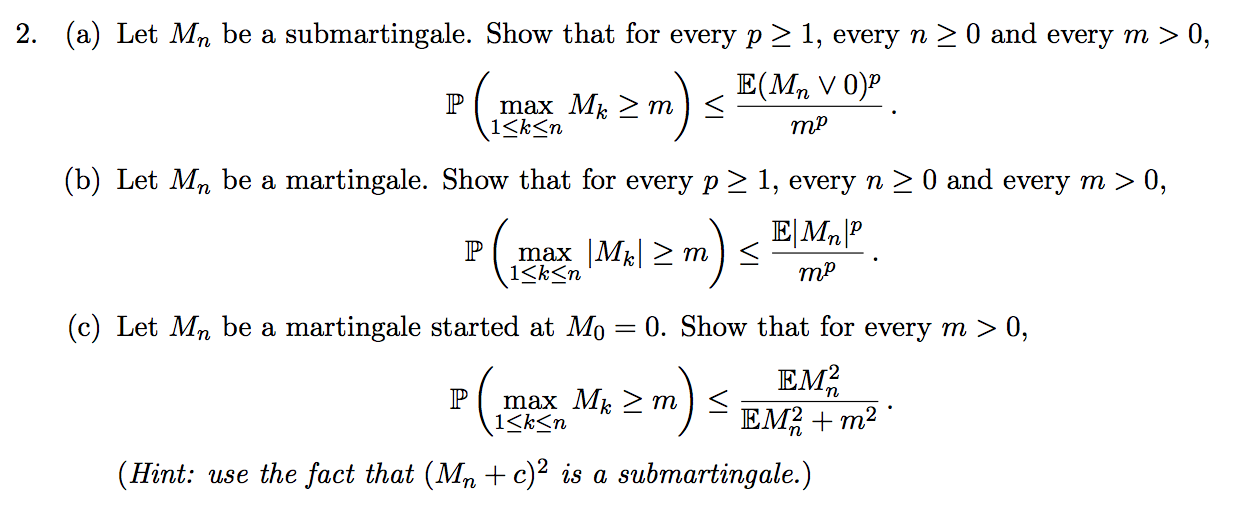
\includegraphics[width=0.7\textwidth]{problim-e12-p2.png}
\end{figure}
\end{question}
\begin{solution} \hfill \\
\textbf{(a)} By convexity, $\{({M_n}^{+})^p\}$ is a submartingale. Then, by Doob's
inequality,
\eQb
\mathbb{P}(\text{max}_{1 \leq k \leq n} M_k \geq m) = 
\mathbb{P}(\text{max}_{1 \leq k \leq n} ({M_k}^{+})^{p} \geq m^{p}) &\leq& 
\dfrac{\mathbb{E}({M_k}^{+})^{p}}{m^p}.
\eQe 

\bigskip

\textbf{(b)} By convexity $\{ | M_n| \}$ is a martingale. By (a),
\eQb
\mathbb{P}(\text{max}_{1 \leq k \leq n} |M_k| \geq m) \leq 
\dfrac{\mathbb{E}[|M_k|^p}{m^p}. 
\eQe

\bigskip

\textbf{(c)} Let $ - c < m$. Then, by hint, and Doob's inequality,
\eQb
\mathbb{P}(\text{max}_{1 \leq k \leq m} M_k \leq m) 
\leq \mathbb{P}(\text{max}_{1 \leq k \leq m} (M_k + c)^2 \geq (m+c)^2) 
\leq \dfrac{\mathbb{E}[M_n^2 + c^2]}{(m+c)^2}.
\eQe 
Viewing the RHS as a function of $c$, denoted as $f$, taking the derivative, 
and setting it equal to 0 give 
\eQb
-2(\mathbb{E}[{M_n}^2] + c^2) + 2c(c+m) = 0 
\eQe
so minimum happens at $c = \dfrac{\mathbb{E}{M_n}^{2}}{m} > 0$. Plugging in the
value of $c$ at the minimum gives the desired inequality. \hfill $\qed$


\end{solution}

\newpage

\begin{question}[3]
\hfill
\begin{figure}[h!]
  \centering
    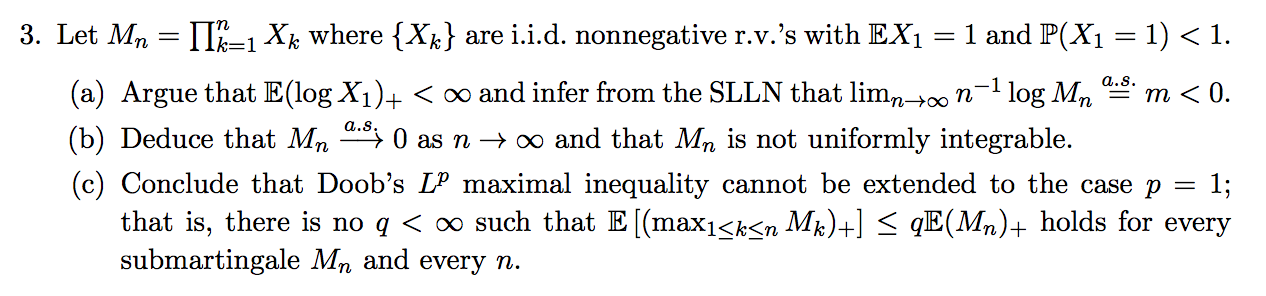
\includegraphics[width=0.7\textwidth]{problim-e12-p3.png}
\end{figure}
\end{question}
\begin{solution} \hfill \\
Define $M_0 = 1$.
Observe that $\{M_n\}$ is a martingale, because, by independence,
\eQb
\mathbb{E}[M_n | \mathscr{F}_{n-1}] = \mathbb{E}[\prod_{k=1}^{n} X_k |
\mathscr{F}_{n-1}] = M_{n-1} \mathbb{E}[X_n|\mathscr{F}_{n-1}] = 
M_{n-1} \mathbb{E}[X_n] = M_{n-1}
\eQe
for any $n \geq 1$. 

\textbf{(a)}
Suppose $\mu = 0$. By chebyshev,
\eQb
\mathbb{E}[\log(X)_{+}] = \int_{0}^{\infty} \mathbb{P}((\log(X) > \lambda) d\lambda
= \int_{0}^{\infty} \mathbb{P}(X > e^{\lambda}) d\lambda 
\leq \int_{0}^{\infty} \dfrac{\mathbb{E}[X]}{e^{\lambda}} d\lambda =
e^{-\lambda}|^{\infty}_{0} = 1. 
\eQe
Hence, by SLLN, $n^{-1}\sum_{k=1}^{n} \log(X_k) = n^{-1}\log(M_n) \to \mu$ almost 
surely, where $\mu = \log(X_1)$.

If $\mu = 0$, then it follows that $X_1$ will be constant, which contradicts the
assumption.


\bigskip

\textbf{(b)} From the convergence in (a),
\eQb
n^{-1}\log(M_n) \leq 2^{-1} \mu 
\eQe
and hence
\eQb
M_n \leq \exp( 2^{-1} \mu n) 
\eQe
almost surely, for all $n$ sufficiently large. Taking $n \to \infty$, shows that
$M_n \to 0$ almost surely. Now,
suppose $\{M_n\}$ is uniformly integrable. Then, $M_n \to 0$ in $L^1$.
However, $\mathbb{E}[M_n] = 1$ for all $n \geq 1$, so we have a contradiction,
and $\{M_n\}$ is not integrable. 

\bigskip

\textbf{(c)} Suppose the $L^p$ maximal inequlaity holds for $p = 1$. Then,
\eQb
\mathbb{E}[\max_{k \leq n} M_k] \leq q\mathbb{E}[M_n] = q \mathbb{E}[M_0] < \infty
\eQe
for some $q < \infty$. Taking $n \to \infty$ shows that
\eQb
\mathbb{E}[\sup_{k} M_k] < \infty
\eQe
which implies that $\{M_n\}$ is U.I, which contradicts $(b)$. So, the maximal
inequality cannot be extended to $p = 1$.
\hfill $\qed$

\end{solution}

\newpage

\begin{question}[4]
\hfill
\begin{figure}[h!]
  \centering
    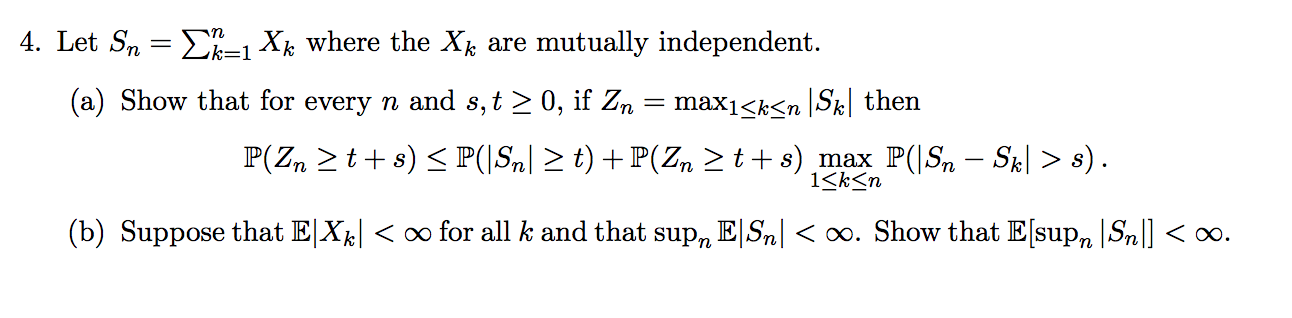
\includegraphics[width=0.7\textwidth]{problim-e12-p4.png}
\end{figure}
\end{question}
\begin{solution} \hfill \\
\textbf{(a)} The idea is to mimic the proof of Levy's maximal inequality.
Set $ E_k = \{ |S_1| < t+s, |S_2| < t + s, ..., |S_{k-1}| < t + s, |S_k| \geq t +s \}$.
Then,
\eQb
\mathbb{P}(Z_n \geq t_s) &=& \mathbb{P}(Z_n \geq t + s, |S_n| \geq t) 
+ \mathbb{P}(Z_n \geq t_s, |S_n| < t) \\ 
&\leq& \mathbb{P}(|S_n| \geq t) + \sum_{k=1}^{n-1} \mathbb{P}(E_k \cap \{|S_n - S_k| > s
\}) \\
&\leq& \mathbb{P}(|S_n| \geq t) + \sum_{k=1}^{n-1}\mathbb{P}(E_k)
\text{max}_{1 \leq k \leq n} \mathbb{P}(|S_n - S_k| > s) \\
&\leq& \mathbb{P}(|S_n| \geq t) + \mathbb{P}(Z_n \geq t+s) 
\text{max}_{1 \leq k \leq n} \mathbb{P}(|S_n - S_k| > s).
\eQe

\textbf{(b)} Observe that
\eQb
\mathbb{E}[\sup_{n} |S_n|] &\leq& \sum_{k=0}^{\infty} \mathbb{P}(\sup_{n} |S_n| 
\geq k) = \sum_{k=0}^{\infty} \mathbb{P}(\sup_{n} Z_n \geq k) \\
&\leq& \sum_{k=0}^{\infty} \sum_{n=0}^{\infty} \mathbb{P}(Z_n \geq k)
\leq 
\sum_{k=0}^{\infty} \sum_{n=0}^{\infty} 
\mathbb{P}(|S_n| \geq k - \dfrac{1}{k}) + \mathbb{P}(Z_n \geq k)
\max_{1 \leq i \leq n} \mathbb{P}(|S_n - S_i| > \dfrac{1}{k}) \\
&\leq& 
\sum_{k=0}^{\infty} \sum_{n=0}^{\infty} 
\mathbb{P}(|S_n| \geq k - \dfrac{1}{k}) + 
\sum_{k=0}^{\infty} \sum_{n=0}^{\infty} 
\mathbb{P}(Z_n \geq k)
\max_{1 \leq i \leq n} \mathbb{P}(|S_n - S_i| > \dfrac{1}{k}) \\
&\leq& \sum_{k=0}^{\infty} \sum_{n=0}^{\infty} 
\mathbb{P}(|S_n| \geq k - \dfrac{1}{k}) + 
\sum_{n=0}^{\infty} \sum_{k=0}^{\infty} 
\mathbb{P}(Z_n \geq k)
\max_{1 \leq i \leq n} \mathbb{P}(|S_n - S_i| > \dfrac{1}{k}). \\
\eQe
For $k = 0$, just take $\dfrac{1}{k}$ in the above expression. Then, from
the fact that $\sup_n \mathbb{E}S_n]$ is bounded, maybe we can deduce
the summability of the RHS.


\end{solution}

\end{document}


